\documentclass[11pt]{article}

\usepackage[margin=1in]{geometry}
\usepackage{titlesec}
\usepackage{enumitem}
\usepackage{xcolor}
\usepackage{tabularx}
\usepackage{booktabs}
\usepackage{fancyhdr}
\usepackage{hyperref}
\usepackage{tikz}
\usetikzlibrary{shapes.geometric, arrows.meta, positioning}

% Define colors
\definecolor{phaseA}{RGB}{70, 130, 180}   % Steel Blue - Design & Planning
\definecolor{phaseB}{RGB}{60, 179, 113}   % Medium Sea Green - Development
\definecolor{phaseC}{RGB}{255, 165, 0}    % Orange - Integration
\definecolor{phaseD}{RGB}{147, 112, 219}  % Medium Purple - Testing & Polish
\definecolor{minesgold}{RGB}{207, 184, 124}
\definecolor{minesblue}{RGB}{33, 49, 77}

% Header/Footer
\pagestyle{fancy}
\fancyhf{}
\fancyhead[L]{\textcolor{minesblue}{\textbf{First Move Robotics}}}
\fancyhead[R]{\textcolor{minesblue}{ProtoFund 2026}}
\fancyfoot[C]{\thepage}
\renewcommand{\headrulewidth}{0.4pt}

% Title formatting
\titleformat{\section}{\Large\bfseries\color{minesblue}}{}{0em}{}[\titlerule]
\titleformat{\subsection}{\large\bfseries\color{minesblue}}{}{0em}{}

\begin{document}

\begin{center}
    {\LARGE\bfseries\textcolor{minesblue}{First Move Autonomous Chess System}}\\[0.5em]
    {\Large 12-Week Development Timeline}\\[1em]
    {\large Colorado School of Mines ProtoFund 2026}\\[0.5em]
    {\normalsize Strydr Silverberg \& Colin Dake}\\[0.5em]
    {\small\textit{Last Updated: \today}}
\end{center}

\vspace{1em}

\section{Project Overview}

First Move Robotics is building an autonomous chess system integrating a computational chess engine with a physical board capable of independent piece manipulation. This timeline accounts for approximately 10--15 hours per week of combined team effort.

\vspace{1em}

\section{Phase Overview}

\begin{center}
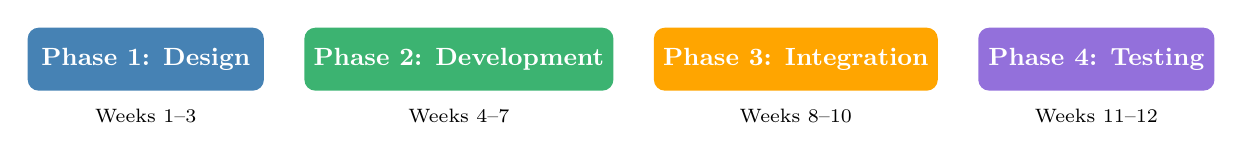
\begin{tikzpicture}[node distance=0.5cm, auto,
    phase/.style={rectangle, rounded corners, minimum width=3cm, minimum height=0.8cm, text centered, font=\small\bfseries, text=white}]
    
    \node[phase, fill=phaseA] (p1) {Phase 1: Design};
    \node[phase, fill=phaseB, right=of p1] (p2) {Phase 2: Development};
    \node[phase, fill=phaseC, right=of p2] (p3) {Phase 3: Integration};
    \node[phase, fill=phaseD, right=of p3] (p4) {Phase 4: Testing};
    
    \node[below=0.1cm of p1, font=\scriptsize] {Weeks 1--3};
    \node[below=0.1cm of p2, font=\scriptsize] {Weeks 4--7};
    \node[below=0.1cm of p3, font=\scriptsize] {Weeks 8--10};
    \node[below=0.1cm of p4, font=\scriptsize] {Weeks 11--12};
    
\end{tikzpicture}
\end{center}

\vspace{1em}

\section{Detailed Weekly Schedule}

%------------------------------------------------------------------------------
\subsection*{\textcolor{phaseA}{Phase 1: Design \& Planning (Weeks 1--3)}}
%------------------------------------------------------------------------------

\noindent\textbf{Week 1: Requirements \& Architecture}
\begin{itemize}[noitemsep, leftmargin=2em]
    \item Define system requirements and success criteria for prototype
    \item Finalize board dimensions, piece design, and movement mechanism approach
    \item Create high-level system architecture diagram
    \item Research and compare actuation methods (XY gantry, electromagnet, robotic arm)
    \item \textit{Deliverable:} Requirements document and architecture diagram
\end{itemize}

\noindent\textbf{Week 2: Component Selection \& Procurement}
\begin{itemize}[noitemsep, leftmargin=2em]
    \item Select microcontroller platform (e.g., Raspberry Pi, Arduino, ESP32)
    \item Identify motors, drivers, sensors, and mechanical components
    \item Create bill of materials (BOM) with suppliers and costs
    \item Place orders for long-lead-time components
    \item Begin CAD modeling of board frame and gantry system
    \item \textit{Deliverable:} Complete BOM with orders placed
\end{itemize}

\noindent\textbf{Week 3: Detailed Design}
\begin{itemize}[noitemsep, leftmargin=2em]
    \item Complete mechanical CAD designs for board structure
    \item Design piece-gripping or electromagnetic mechanism
    \item Create wiring schematics and PCB layout (if custom board needed)
    \item Define software module interfaces and communication protocols
    \item Set up version control repository and project management tools
    \item \textit{Deliverable:} Complete CAD files and electrical schematics
\end{itemize}

\vspace{0.5em}

%------------------------------------------------------------------------------
\subsection*{\textcolor{phaseB}{Phase 2: Parallel Development (Weeks 4--7)}}
%------------------------------------------------------------------------------

\noindent\textbf{Week 4: Foundation Build}
\begin{itemize}[noitemsep, leftmargin=2em]
    \item \textbf{Hardware:} Begin frame construction; assemble linear motion components
    \item \textbf{Software:} Set up development environment; implement basic UCI protocol
    \item Verify motor drivers and test basic motion control
    \item \textit{Deliverable:} Partial frame assembly; motor control proof-of-concept
\end{itemize}

\noindent\textbf{Week 5: Core Subsystems}
\begin{itemize}[noitemsep, leftmargin=2em]
    \item \textbf{Hardware:} Complete gantry assembly; mount motors and belts/leadscrews
    \item \textbf{Software:} Implement board state representation and move validation
    \item Begin piece detection system (reed switches, hall effect sensors, or vision)
    \item \textit{Deliverable:} Functional XY motion; basic chess logic operational
\end{itemize}

\noindent\textbf{Week 6: Piece Manipulation}
\begin{itemize}[noitemsep, leftmargin=2em]
    \item \textbf{Hardware:} Install and test piece-gripping mechanism
    \item \textbf{Software:} Develop motion planning for piece pickup, movement, and placement
    \item Implement coordinate calibration routines
    \item Buffer week for catching up on delayed components or debugging
    \item \textit{Deliverable:} System can physically move a single piece between squares
\end{itemize}

\noindent\textbf{Week 7: Chess Engine Integration}
\begin{itemize}[noitemsep, leftmargin=2em]
    \item Integrate engine with physical control system
    \item Implement move translation layer (algebraic notation $\rightarrow$ motor commands)
    \item Add piece capture handling (remove captured pieces from board)
    \item Begin basic game flow: detect human move, compute response, execute move
    \item \textit{Deliverable:} Engine-controlled piece movement demonstrated
\end{itemize}

\vspace{0.5em}

%------------------------------------------------------------------------------
\subsection*{\textcolor{phaseC}{Phase 3: System Integration (Weeks 8--10)}}
%------------------------------------------------------------------------------

\noindent\textbf{Week 8: Full Game Loop}
\begin{itemize}[noitemsep, leftmargin=2em]
    \item Implement complete game state machine (start, play, end-game detection)
    \item Add castling and en passant move handling
    \item Integrate piece detection with move validation
    \item Test human vs.\ engine gameplay for basic positions
    \item \textit{Deliverable:} Complete game playable from starting position
\end{itemize}

\noindent\textbf{Week 9: User Interface \& Feedback}
\begin{itemize}[noitemsep, leftmargin=2em]
    \item Add user feedback mechanisms (LEDs, display, or audio)
    \item Implement difficulty level selection
    \item Create simple interface for game start/reset
    \item Handle error states (illegal moves, piece misplacement)
    \item \textit{Deliverable:} User-friendly interaction layer
\end{itemize}

\noindent\textbf{Week 10: Reliability \& Edge Cases}
\begin{itemize}[noitemsep, leftmargin=2em]
    \item Stress test mechanical system for repeated moves
    \item Handle edge cases: pawn promotion, stalemate, checkmate detection
    \item Implement graceful error recovery
    \item Optimize motion paths for speed and reliability
    \item \textit{Deliverable:} Robust system handling all standard chess scenarios
\end{itemize}

\vspace{0.5em}

%------------------------------------------------------------------------------
\subsection*{\textcolor{phaseD}{Phase 4: Testing \& Documentation (Weeks 11--12)}}
%------------------------------------------------------------------------------

\noindent\textbf{Week 11: Testing \& Refinement}
\begin{itemize}[noitemsep, leftmargin=2em]
    \item Conduct full system testing with multiple complete games
    \item Identify and fix mechanical reliability issues
    \item Fine-tune motor speeds, acceleration profiles, and timing
    \item Begin documentation of system design and operation
    \item \textit{Deliverable:} Reliable prototype; draft documentation
\end{itemize}

\noindent\textbf{Week 12: Documentation \& Presentation}
\begin{itemize}[noitemsep, leftmargin=2em]
    \item Complete technical documentation
    \item Prepare demonstration materials and presentation
    \item Record demonstration video
    \item Create user manual for prototype operation
    \item Final system cleanup and packaging
    \item \textit{Deliverable:} Complete prototype ready for ProtoFund presentation
\end{itemize}

\vspace{1em}

\section{Minimum Viable Prototype (MVP) Criteria}

The prototype will be considered successful if it demonstrates:

\begin{enumerate}[noitemsep]
    \item Physical board with functional XY positioning system
    \item Reliable piece manipulation (pickup, move, place)
    \item Human move detection via sensors
    \item Engine integration with legal move generation
    \item Completion of at least one full game against a human opponent
\end{enumerate}

\vspace{1em}

\section{Task Division}

\begin{tabularx}{\textwidth}{l X X}
\toprule
\textbf{Phase} & \textbf{Colin Dake (Hardware Focus, Software and Hardware Integration)} & \textbf{Strydr Silverberg (Software Focus, Software and Hardware Integration)} \\
\midrule
Weeks 1--3 & Mechanical design, CAD, BOM & System architecture, interface design \\
Weeks 4--7 & Frame construction, wiring, motors & Chess engine, motion control software \\
Weeks 8--10 & Sensor integration, calibration & Game logic, UI, error handling \\
Weeks 11--12 & Mechanical refinement & Documentation, testing scripts \\
\bottomrule
\end{tabularx}

\vspace{2em}

\end{document}
